%
% general.tex -- 
%
% (c) 2019 Prof Dr Andreas Mueller
%
\section{The general case}
\rhead{The general case}
We now want to solve the general case of the problem
\[
\begin{aligned}
\Delta u&=f&&\text{in $\Omega$}\\
u&=g&&\text{auf $\partial\Omega$}
\end{aligned}
\]
using an integral formula of the kind
\eqref{greenformula}.
Following the one dimensional case, we are looking for a particular
solution $G(x,\xi)$ for the problem with a $\delta$-distribution on
the right hand side.
Once such a solution is found, we can find solutions for the general
problem using an integral formular.

\subsection{A particular solution}
\rhead{Particular solution}
The one-dimensional sample problem suggests that there is a function
$\sigma(x,\xi)$, which allows to find a particular solution of the
Laplace equation using the integral
\begin{equation}
u_p(x)=\int_\Omega \sigma(x,\xi)  f(\xi)\,d\xi.
\label{singulaereloesunglaplace}
\end{equation}
This particular solution does not need to satisfy the boundary conditions,
we just require that $\Delta u=f$ holds.

The solution $\sigma$ does not have to depend on the shape of the domain,
as it does not have to respect any boundary conditions,
but it will change with the dimension $n$.
If we choose the right hand side $f$ to be a $\delta$ distribution in the
point $y$, then
\[
u(x)
=
\int_\Omega \sigma(x,\xi)\delta(\xi - y)\,d\xi
=
\sigma(x,y).
\]
Thus the partial function $x\mapsto \sigma(x,y)$ satisfies the equation
$\Delta \sigma(x,y)=0$ for all points in ${\mathbb R}^n\setminus\{y\}$.
The function $\sigma$ thus is a harmonic function in the set
$\mathbb R^n\setminus\{y\}$.

Determining the function $\sigma(x,y)$ is a bit tedious, we just give the
result.
We find\footnote{%
This solution can be found using the following argument.
First the solution should only depend on the distance $|x-\xi|$, which
means we can assume without losing any generality that $\xi=0$.
As $\Delta u=\operatorname{div}\operatorname{grad}u$ we  conclude using
Gauss' theorem that
\begin{align*}
1&=\int_{B_r^n} \Delta u(x)\,d\mu(x)
=
\int_{B_r^n} \operatorname{div}\operatorname{grad} u(x)\,d\mu(x)
=\int_{S_r^{n-1}}\operatorname{grad}u(x)\cdot dn
\\
&=\int_{S_r^{n-1}}|\operatorname{grad}u(x)|\,d\mu(x)
=\mu(S_r^{n-1})\left|\frac{d}{dr}u(r)\right|
\\
\Rightarrow\qquad\frac{d}{dr}u(r)
&=\frac1{\mu(S_r^{n-1})}
=\frac1{\mu(S_1^{n-1})r^{n-1}}.
\end{align*}
For $n=2$ we have
$\mu(S_r^1)=2\pi r$, which implies
\[
u'(r)=\frac1{2\pi r}\quad\Rightarrow\quad u(r)=\frac1{2\pi}\log|r|.
\]
For $n\ge 3$ we get
\[
u'(r)=\frac1{\mu(S^{n-1})}r^{1-n}\quad\Rightarrow\quad u(r)=\frac1{\mu(S^{n-1})}\cdot \frac1{2-n}r^{2-n}.
\]
}
\begin{equation}
\sigma(x,\xi)=
\begin{cases}
\displaystyle \frac12|x-\xi|
&\qquad \text{für $n=1$}
\\
\\
\displaystyle \frac1{2\pi}\log|x-\xi]
&\qquad \text{für $n=2$}
\\
\\
\displaystyle -\frac1{4\pi}\frac1{|x-\xi|}
&\qquad \text{für $n= 3$}
\\
\\
\displaystyle \frac1{(2-n)\mu(S^{n-1})}|x-\xi|^{2-n}
&\qquad \text{für $n\ge 3$}
\end{cases}
\end{equation}
For $n=1$ we already have determined this function in \eqref{n1sigma}.
By carefully performing all these derivatives we can verify
that these functions are in fact solutions and that
\eqref{singulaereloesunglaplace} is particular solution of
Laplace equation.

\subsection{Green's function}
The propsed $\sigma$ is of course not the only function for which
the formula \eqref{singulaereloesunglaplace} will give a particular solution.
By adding any function $h(x,\xi)$ which is harmonic as a function of $x$
the integral
\[
u(x)=\int_{\Omega}\sigma(x,\xi)f(\xi)\,d\xi-\int_{\Omega}h(x,\xi)f(\xi)\,d\xi
\]
will also be a solution of
\eqref{elliptisch:laplaceequation}.
In particular we can choose $h(x,\xi)$ in such a way that
the partial function
$x\mapsto h(x,\xi)$
solves the boundary value problem
\[
\begin{aligned}
\Delta_x h(x,\xi)&=0&&x\in\Omega\\
h(x,\xi)&=\sigma(x,\xi)&&x\in\partial\Omega.
\end{aligned}
\]
The function $h$ then has the same boundary values as $\sigma$.
Consequently the difference $\sigma(x,\xi)-h(x,\xi)$ is a function
that vanishes on the boundary $\partial\Omega$.
The solution $u(x)$ found using \eqref{singulaereloesunglaplace}
then also vanishes on the boundary.
We set
\[
G(x,\xi)=\sigma(x,\xi)-h(x,\xi)
\]
and call this the Green's function for the Poisson problem on the
domain $\Omega$.

\begin{satz}If $\Omega$ is a domain on which the Poisson problem
has unique solutions, then there is a function $G(x,\xi)$,
which, as a function $x$, solves the equation
\[
\Delta G(x,\xi)=\delta(x-\xi)
\]
with homogenous boundary conditions.
\end{satz}

Note that this theorem guarantees the existence of Green's function 
but does not provide a method to obtain it.
Green's function deends only on the shape of the domain, not on
the actual boundary condtions.
Since there are domains where the Poisson problem with Dirichlet
boundary conditions cannot be solved in a unique way, the theorem
needs to require this as a precondition.

Green's function for the Poisson problem solves the problem
not only for homogeneous ($g=0$) boundary conditions, sondern
for any boundary values $g\ne 0$:

\begin{satz}[Solution of Poisson problem with Dirichlet boundary conditions]
\label{dirichletloesung}
If $G$ is Green's function for the Poisson problem with Dirichlet
boundary values on the domain $\Omega$, then
\[
u(x)
=
\int_{\Omega}G(x,\xi)f(\xi)\,d\mu(\xi)
+
\int_{\partial\Omega}g(\xi)\operatorname{grad}_\xi G(x,\xi)\cdot dn
\]
is the solution for the same problem with arbitrary boundary values
\eqref{dirichletrandbedingung}.
\end{satz}

Note that is very much in line with what we have found for the one
dimensional case.
The terms of \eqref{elliptic:greendiff} containing the derivatives
of $G$ can be considered as the integral of the gradient of $G$
over the bounary of the interval, which would be computed as a sum
of the values in the boundary points.

\begin{proof}
We already know that the integral over $\Omega$ is a solution of the
inhomogeneous partial differential equation with homogeneous boundary
conditions.
What remains is to show that the second term is a harmonic function,
i.~e.~it solves the homogeneous differential equation,
with boundary values $g$.

For this proof we need the following identity
\begin{align*}
\operatorname{div}(u\operatorname{grad}v)
&=
\sum_i\partial_i(u\partial_iv)
\\
&=\sum_i(\partial_iu)(\partial_iv)+\sum_iu\partial_i^2v
\\
&=\operatorname{grad}u\cdot\operatorname{grad}v+u\Delta v,
\end{align*}
from which we can derive
\[
u\Delta v-v\Delta u
=
\operatorname{div}(u\operatorname{grad}v-v\operatorname{grad}u).
\]

We apply these identities to the function $u(\xi)$ and 
to Green's function $\xi\mapsto v(\xi)=G(x,\xi)$:
\[
u(\xi)\Delta G(x,\xi)-G(x,\xi)\Delta u
=
\operatorname{div}(u\operatorname{grad}G(x,\xi)-G(x,\xi)\operatorname{grad}u)
\]
Integrating both sides over $\Omega$ and applying Gauss' theorem to
the right hand side gives
\begin{align*}
\int_{\Omega}u(\xi)\delta(\xi - x)-G(x,\xi)f(\xi)\,d\mu(\xi)
&=
\int_{\Omega}\operatorname{div}(u(\xi)\operatorname{grad}G(x,\xi)-G(x,\xi)\operatorname{grad}u)\,d\mu(\xi)
\\
u(x)-\int_{\Omega}G(x,\xi)f(\xi)\,d\mu(\xi)
&=\int_{\partial \Omega}u(\xi)\operatorname{grad}G(x,\xi)-G(x,\xi)\operatorname{grad}u(\xi)\cdot dn
\end{align*}
The second term on the right vanishes becuase $G(x,\xi)$ was chosen so
that the boundary values vanish.
In the left term we can replace $u(\xi)$ by the boundary values $g(\xi)$.
What remains is
\[
u(x)
=
\int_{\Omega}G(x,\xi)f(\xi)\,d\mu(\xi)
+
\int_{\partial\Omega}g(\xi)\operatorname{grad}G(x,\xi)\cdot dn,
\]
as claimed.
\end{proof}

\subsection{Application}
\rhead{Application}
\begin{figure}
\begin{center}
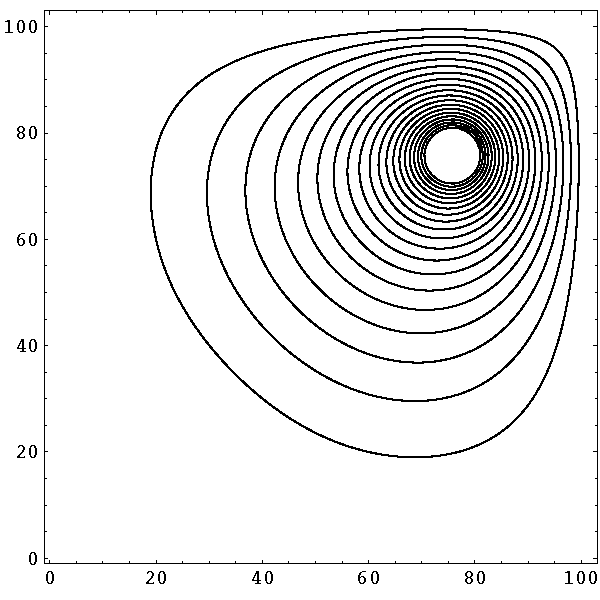
\includegraphics[width=0.8\hsize]{../common/graphics/neilcontour}
\end{center}
\caption{Level lines\label{neilcontour}}
\end{figure}
\begin{figure}
\begin{center}
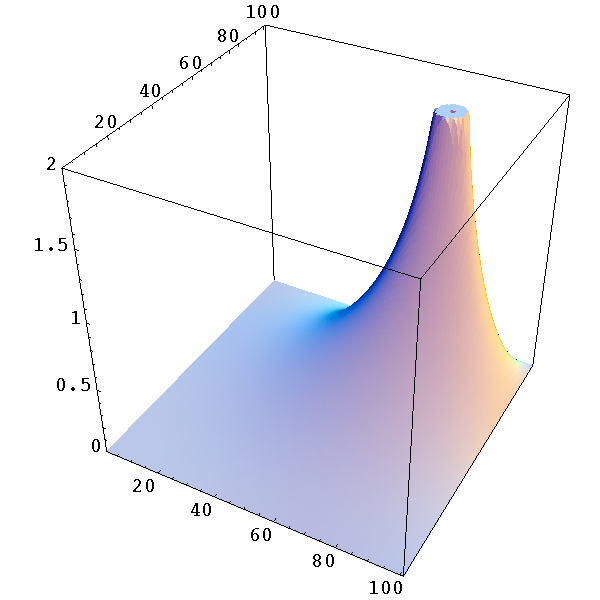
\includegraphics[width=0.8\hsize]{../common/graphics/neilloesung}
\end{center}
\caption{Potential surface\label{neilloesung}}
\end{figure}
This example illustrates how the ideas in this section can be used
to solve some practical problems at least using some numerical tool.

{\parindent 0pt
\medskip
{\bf Problem:}
The boundary of an electricaly conducting rectangular plate is connected
to the negative terminal of a battery and at the point
$x_0\in\mathbb R^2$ in the interior of the plate, the other terminal
of the battery is connected.
Compute the potential at any point $x$ of the plate with respect to
the boundary.

\medskip
}
The potential
$u(x,y)$
we are looking for is the solution of the equation
\[
\Delta u=\delta(x-x_0)
\]
with boundary values
\[
u(x)=0.
\]
Numerical computation of the solution in the vicinity of the point $x_0$
is very imprecise.
This motivates the following procedure.
The function $\sigma(x,x_0)$ is a harmonic function outside $x_0$,
\[
\Delta\sigma(x,x_0)=\delta(x-x_0)
\]
So appart from the boundary values that are not correct it could be
a solution.
So the next step is to fix the boundary values of this partial solution.
For this we solve the boundary value problem
\begin{align*}
\Delta h(x)&=0&&x\in\Omega\\
h(x)&=\sigma(x,x_0)&&x\in\partial\Omega,
\end{align*}
which can be done efficiently with existing software.
E.~g.~we could use the mean value property to be discussed later in this
chater to numerically compute such a solution.
Then the function
\[
u(x)=\sigma(x,x_0)-h(x)
\]
is a solution of the original problem.
The level lines of this solutions and the potential surface of $u(x)$ is
shown in figures~\ref{neilloesung} and \ref{neilcontour}.

